\section{Implementation in \pkg{gretl}}\label{sec:BACE_implementation}
In this section, we describe the code of the \pkg{BACE}
package. First, we will characterize our code and the use
of both: the command line and the GUI interfaces, then we
will present some examples of using the \pkg{BACE}.
Finally, we will show the outputs that are returned.

\subsection{The core of the \pkg{BACE} code}
The \pkg{BACE} package consists of 4 public and 14
private functions. The name of each function starts
with the \cmd{BACE\_} prefix. The public functions are:
\begin{enumerate}
	\item \cmd{BACE()}~see~\ref{sec:BACE()}
	\item \cmd{BACE\_GUI()}~see~\ref{sec:BACE_GUI()}
	\item \cmd{BACE\_Print()}~see~\ref{sec:BACE_Print()}
	\item \cmd{BACE\_Plot()}~see~\ref{sec:BACE_Plot()}
\end{enumerate}

\subsubsection{\cmd{BACE()}}\label{sec:BACE()}
This is a core package function which runs and controls
the main loop. As a consequence, it is a prime interface
to the \pkg{BACE} package. The \cmd{BACE()} function
returns a bundle with all information needed to print
and/or plot results anytime. One can print the results
by calling \cmd{BACE\_Print()} or plot graphs by calling
\cmd{BACE\_Plot()}. The signature of \cmd{BACE()}
function is as follows:
\begin{lstlisting}
function bundle BACE (series Y "Dependent variable",
 list X_list "List of indenpendent variables (X)",
 bundle Options[null])	
\end{lstlisting}
The first two options are mandatory, while the last one
is an optional collection of additional arguments. Those
arguments are defined with the following default values:
\begin{lstlisting}
scalar Options["Y_AR_p"] = 0
scalar Options["with_const"] = 1
scalar Options["model_prior"] = 2
scalar Options["avg_model_size"] = avg_model_size_tmp
scalar Options["alpha"] = 0.6
scalar Options["Nrank"] = xmin(2^(k+Y_AR_p_tmp-1), 40)
scalar Options["do_joint"] = 0
scalar Options["Npredict"] = 0
scalar Options["Nrep"] = Nrep
scalar Options["burn"] = 10
scalar Options["verbosity"] = 2
scalar Options["show_progress"] = do_show_progress
scalar Options["do_plot"] = do_plot_tmp
string Options["model_type"] = "linear"
scalar Options["data_trans"] = 0
scalar Options["bic_type"] = 1
scalar Options["hyperparameter"] = 0.5 # gamma for EBIC
scalar Options["binary_threshold"] = 0.5
scalar Options["_gui"] = 0	
\end{lstlisting}
where \textit{k} stands for the number of independent variables,
\lstinline!scalar avg_model_size! is calculated according to
the following formula:
\begin{equation}
	\texttt{\lstinline!avg\_model\_size!} = \left\{
	\begin{array}{lll}
		\textrm{\lstinline!(k + Y\_AR\_p\_tmp)/2!} & \mathrm{if} & \textrm{\lstinline!with_const \!= 2!},\\
		\textrm{\lstinline!(k + Y\_AR\_p\_tmp + 1)/2!} & \mathrm{elsewhere}, &\\
	\end{array}
	\right.
	\label{eq:avg_model_size_setup}
\end{equation}
\lstinline!scalar Nrep! takes the following values:
\begin{equation}
	\texttt{\lstinline!Nrep!} = \left\{
	\begin{array}{ccl}
		10^3 & \mathrm{if} & k \leq 10,\\
		10^4 & \mathrm{if} & k \in [11;15],\\
		10^5 & \mathrm{if} & k \in [16;19],\\
		10^6 & \mathrm{if} & k \geq 20,\\
	\end{array}
	\right.
	\label{eq:Nrep_setup}
\end{equation}
\lstinline!scalar show_progress! takes the following values:
\begin{equation}
	\texttt{\lstinline!show\_progress!} = \left\{
	\begin{array}{cll}
		1 & \mathrm{if} & \textrm{\lstinline!$sysinfo!\texttt{\small.gui\_mode}},\\
		0 & \mathrm{elsewhere}, &\\
	\end{array}
	\right.
	\label{eq:show_progress_setup}
\end{equation}
and \lstinline!scalar do_plot! takes the following values:
\begin{equation}
	\texttt{\lstinline!do\_plot!} = \left\{
	\begin{array}{cll}
		1 & \mathrm{if} & \textrm{\lstinline!$sysinfo!\texttt{\small.gui\_mode}},\\
		0 & \mathrm{elsewhere}. &\\
	\end{array}
	\right.
	\label{eq:do_plot_setup}
\end{equation}
Most of the optional parameters listed above are of
numerical type and they may be gathered into following
groups according to what kind of numbers they can take%
\footnote{Note, that the \lstinline!scalar _gui! is
	for internal use only and must not be modified
	by user at any rate.}:
\begin{enumerate}
	\item Integers: \lstinline!Y_AR_p!, \lstinline!with_const!,
		\lstinline!model_prior!, \lstinline!Nrank!, \lstinline!do_joint!,
		\lstinline!Npredict!, \lstinline!Nrep!, \lstinline!burn!,
		\lstinline!verbosity!, \lstinline!data_trans!, \lstinline!bic_type!.
	\item Booleans: \lstinline!show_progress!, \lstinline!do_plot!.
	\item Scalars: \lstinline!avg_model_size!, \lstinline!alpha!,
		\lstinline!binary_threshold!.
\end{enumerate}
Optional parameters control the following package options:
\begin{enumerate}
	\item \textbf{Y\_AR\_p}: autoregression order of variable Y.
	\item \textbf{with\_const}: whether we include constant term
		in each estimated model?; possible values are: 0---without
		constant, 1---constant is always included, 2---constant
		may be dropped.
	\item \textbf{model\_prior}: model prior distribution to use;
		possible values are: 0---none, 1---Binomial, 2---Beta-Binomial.
	\item \textbf{avg\_model\_size}: expected average model size
		for model prior.
	\item \textbf{alpha}: significance level for the initial model.
	\item \textbf{Nrank}: number of top ranked models.
	\item \textbf{do\_joint}: do we perform jointness analysis?;
		possible values are: 0---none, 1---Doppelhofer-Weeks
		Measure (DW1), 2---Doppelhofer-Weeks Measure (DW2),
		3---Ley-Steel Measure (LS1), 4---Ley-Steel Measure (LS2),
		5---Strachan Measure, 6---Yule's Q Measure (YQ),
		7---Modified Yule's Q Measure (YQM).
\end{enumerate}

\subsubsection{\pkg{BACE\_GUI()}}\label{sec:BACE_GUI()}
The \cmd{BACE\_GUI()} is a wrapper to \cmd{BACE()}
interface and takes the following parameters:
\begin{itemize}
	\item \textbf{Dependent variable} as series [required].
	\item \textbf{Y lags} as integer with zero (only for time-series).
	\item \textbf{List of independent variables (X)} as list [may be null].
	\item \textbf{Constant in model} as integer [required]:
	\begin{enumerate}
		\item Never -- all models without constant,
		\item Always -- all models with constant,
		\item Can be dropped -- constant may be removed from or added to any model.
	\end{enumerate}
	\item \textbf{Model prior} as integer [required]:
	\begin{enumerate}
		\item Binomial -- binomial distribution,
		\item Beta-Binomial -- beta-binomial distribution.
	\end{enumerate}
	\item \textbf{Prior average model size} as scalar with zero [required].
	\item \textbf{Significance level for the initial model} as scalar from $(0,1)$
	[required].
	\item \textbf{Number of the top ranked models} as integer [required].
	\item \textbf{Jointness analysis} as integer with zero [required]%
	\footnote{Values $\pm 999.000000$ should be interpreted as $\pm \infty$.}:
	\begin{enumerate}
		\item None -- we do not perform any jointness analysis,
		\item Ley-Steel Measure -- we perform jointness analysis with Ley-Steel measure,
		\item Doppelhofer-Weeks Measure -- we perform jointness analysis with Doppelhofer-Weeks measure.
	\end{enumerate}
	\item \textbf{Number of out-of-sample forecasts} as integer with zero [required].
	\item \textbf{Total number of replications} as integer [required].
	\item \textbf{Percentage of burn-in draws} as integer from (0, 99) [required].
	\item \textbf{Verbosity} as integer [required].
	\item \textbf{Show overall progress} as Boolean.
\end{itemize}


\subsection{The GUI way}
Once you start \cmd{gretl}, you must open a data file and then you can
load the relevant \cmd{BACE} package from the \cmd{gretl} server. In the main
window, go to File $\rightarrow$ Function packages $\rightarrow$ On server
heading. By selecting \cmd{BACE}, you will download the package on your
local machine. Next, go to File $\rightarrow$ Function packages $\rightarrow$
On local machine and by selecting BACE from the list open a window similar
to the one shown in Figure~\ref{fig:Main window for BACE}:

\begin{figure}[h!]
	\centering
	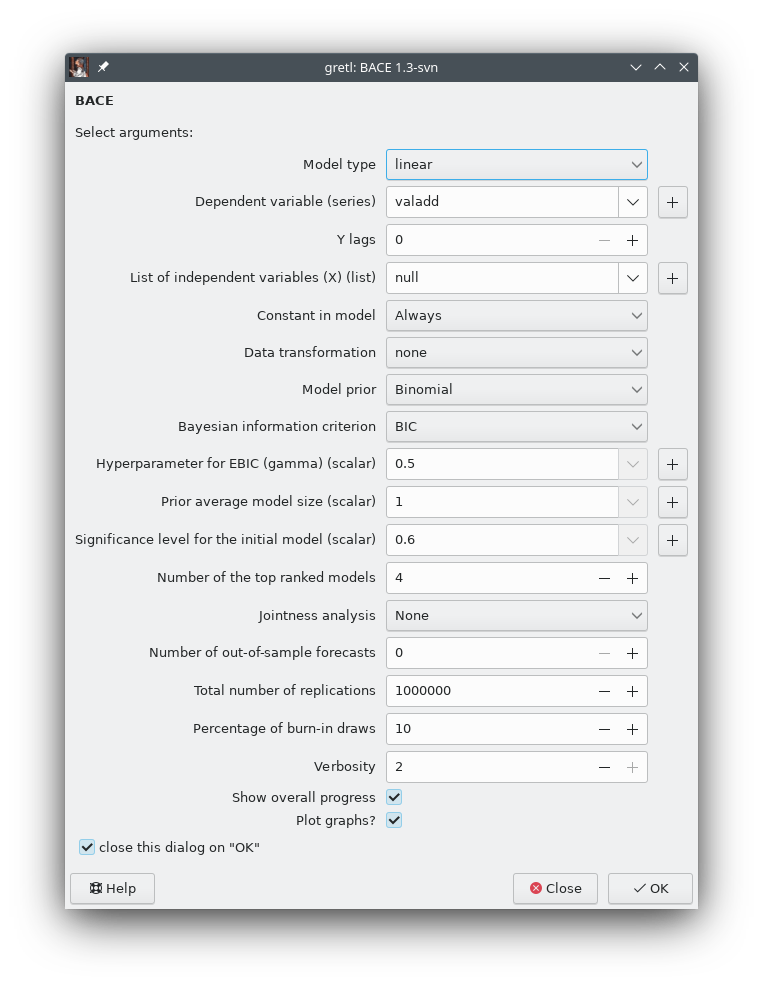
\includegraphics[width=0.7\columnwidth, keepaspectratio]{PNG/BACE_main_window}
	\caption{Main window for \cmd{BACE}.}
	\label{fig:Main window for BACE}
\end{figure}

According to Figure~\ref{fig:Main window for BACE}, we can specify the following
entries in the GUI \cmd{BACE} window\label{text:module_parameters}
\begin{itemize}
	\item \textbf{Model type} -- What kind of modeling should be
		should be performed?
	\item \textbf{Dependent variable} -- The dependent variable.
	\item \textbf{Y lags} -- number of lags for dependent variable
		(for time-series only).
	\item \textbf{List of independent variables}
		-- List of all independent variables (including lagged series).
	\item \textbf{Constant in model} -- Do we include intercept?
		It can be: always, never or can be dropped.
	\item \textbf{Bayesian information criterion} -- Version of BIC to
		be used.
	\item \textbf{Jointness analysis} -- If \cmd{None} (the default),
		the jointness analysis is omitted. Alternatively, one can
		choose one of the 7 available jointness measures.
	\item \textbf{Number of out-of-sample forecasts} -- Defines the
		total number of out-of-sample forecasts of the dependent variable.
	\item \textbf{Verbosity} -- An integer value of 1 or 2; the default
		is 2, so a more detailed description of the	analysis is provided
		(initial model, speed of convergence, estimation results for top
		ranked models).
	\item \textbf{Show overall progress} -- The progress bar is printed.
	\item \textbf{Plot graphs?} -- Shall we produce graphs?
\end{itemize}

\subsection{The script way}
\subsubsection{Script}
The \cmd{BACE} package can also be used inside \proglang{Hansl} scripts.
A very minimal code could be as follows:
%
\begin{lstlisting}
open greene9_1.gdt
include BACE.gfn

list greene = capital labor nfirm

BACE(valadd, greene)
\end{lstlisting}
The above code triggers BACE analysis with default option
described on page~\pageref{sec:default_option_bundle}.
On contrary, the corresponding ''big call'', i.e. with
setting all possible parameters, would be as follows:
\begin{lstlisting}
bundle opts = defbundle("model_prior", 2, "avg_model_size", 1.5, \
  "alpha", 0.6, "Nrank", 4, "do_joint", 0, "Npredict", 0, \
  "Nrep", 1000, "burn", 10, "verbosity", 2, "show_progress", 1, \
  "do_plot", 1, "model_type", "linear", "const_type", 1, \
  "bic_type", 1, "data_trans", 0)

BACE(valadd, greene, opts)
\end{lstlisting}

or alternatively with the new syntax for creating a bundle
on-the-fly:
\begin{lstlisting}
	BACE(valadd, greene, _(model_prior=2, avg_model_size=1.5, \
	alpha=0.6, Nrank=4, do_joint=0, Npredict=0, Nrep=1000, \
	burn=10, verbosity=2, show_progress=1, do_plot=1, \
	model_type="linear", const_type=1, bic_type=1, data_trans=0))
\end{lstlisting}
Since some parameters in option bundle are over-loadable,
the equivalent call looks like this:
\begin{lstlisting}
	BACE(valadd, greene, _(model_prior="beta-binomial", \
	avg_model_size=1.5, alpha=0.6, Nrank=4, do_joint="none", \
	Npredict=0, Nrep=1000, burn=10, verbosity=2, show_progress=1, \
	do_plot=1, model_type="linear", const_type="always", \
	bic_type="bic", data_trans="none"))
\end{lstlisting} 
The above example consists of three blocks.

\begin{lstlisting}
	open greene9_1.gdt
	include BACE.gfn
	set seed 1000000
	
	list greene = capital labor nfirm
	
	scalar model_type = 1
	scalar y_lags = 0
	scalar with_const = 1
	scalar data_trans = 0
	scalar model_prior = 1
	scalar bic_type = 1
	scalar hyperparameter = 0
	scalar prior_avg_model_size = 1.5
	scalar alpha = 0.6
	scalar top_ranked_model = 4
	scalar joint = 1
	scalar forecasts = 0
	scalar Nrep = 2000
	scalar Nburn = 10
	scalar verbosity = 1
	scalar progress = 1
	scalar plots = 1
	
	BACE_GUI(model_type, valadd, y_lags, greene, with_const,\
	data_trans, model_prior, bic_type, hyperparameter,\
	prior_avg_model_size, alpha, top_ranked_model, joint,\
	forecasts, Nrep, Nburn, verbosity, progress, plots)
\end{lstlisting}

The above example consists of three blocks.
The first block is just opening of the so called \cmd{greene9\_1}
dataset, which is bundled in every standard gretl installation.
This dataset contains cross-sectional data on manufacturing
of transportation equipment presented as Table 9.1 in
\cite{greene_Econometric_A}%
\footnote{This dataset is also available at link
	\url{http://people.stern.nyu.edu/wgreene/Text/Edition7/TableF7-2.txt}.}.
We also set the seed in order to exact reproduction of the results.

The second block is the definition of the \cmd{greene} list which
contains three independent variables available in the \cmd{greene9\_1} dataset.

The third block contains the definition for Bayesian Averaging of Classical
Estimates analysis: no lags for Y variable (not applicable since we have
cross-sectional data), constant always included, binomial model prior,
prior average model size set to 1.5 (which means that we have uniform model prior),
significance level for the initial model set to 0.6, 4 top ranked models,
jointness analysis with Ley-Steel Measure, without out-of-sample predictions,
10000 replications with 10\% burn-in draws, basic output (verbosity set to 1)
and progress overall progress is printed.

Suppose we want to run the same analysis but following
Occam's razor principle. The simplest way is setting the prior
average model size to 1. We also want to have ''random'' constant,
i.e. intercept can be dropped in any model. We also want to save
results of the BACE analysis in the bundle \cmd{results\_b},
the code should be as follows:
\begin{CodeChunk}
	\begin{CodeInput}
		prior_avg_model_size = 1
		with_const = 2
		
		results_b = BACE_GUI(valadd, y_lags, greene, with_const, model_prior, 
		prior_avg_model_size, alpha, top_ranked_model, joint, forecasts,
		Nrep, Nburn, verbosity, progress)
	\end{CodeInput}
\end{CodeChunk}

Suppose we want to calculate Doppelhofer-Weeks Measure instead of
already computed Ley-Steel Measure. Since the type of jointness measure
is controlled by \cmd{do\_join} field in the result bundle, the only thing
we have to do is to set the value of \cmd{do\_join} to 2 and print BACE
results again. The code should be as follows:
\begin{CodeChunk}
	\begin{CodeInput}
		results_b.do_joint = 2
		BACE_Print(&results_b)
	\end{CodeInput}
\end{CodeChunk}


\subsection{Output}\label{sec:outputs}
\textcolor{red}{\textbf{Outdated!!!}}\newline
If you select the appropriate entries in the GUI \cmd{BACE} window,
our package returns: Posterior Inclusion Probabilities (PIP), the
averages of the posterior means and standard deviations of parameters
(``Mean'' and ``Std.Dev.'', respectively) and the posterior mean and
standard deviation of each coefficient conditional on the variable
being included in the model (``Cond.Mean'' and
``Cond.Std.Dev.''). Furthermore, the package also returns the
predictive results for the dependent variable (``Mean'' and
``Std.Dev.'').

Let us consider the data used in previous example
(\cmd{australia.gdt}).  This dataset contains the Australian macro
data used in \cite{Johansen1995Likelihood} and originally supplied by
Tony Hall.  The variables used in the text are:
\begin{itemize}
	\item lpau -- log of Australian CPI (dependent variable),
	\item lpus -- log of US CPI,
	\item le -- log of exchange rate (price of US dollars in Aus. dollars),
	\item iau2 -- 5-year Treasury bond rate, Australia,
	\item ius2 -- 5-year Treasury bond rate, USA. 
\end{itemize}
Suppose we want to perform BACE analysis up to $ADL(2,2)$ specification,
i.e. all possible combinations from $ADL(0,0)$ to $ADL(2,2)$.
The example script would be as follows:

\begin{CodeChunk}
	\begin{CodeInput}
		set verbose off
		include BACE.gfn
		open australia.gdt
		genr time
		
		# We create lagged values
		adl_lags = 2
		lags(adl_lags, ius2)
		lags(adl_lags, iau2)
		lags(adl_lags, e2)
		lags(adl_lags, lpus)
		lags(adl_lags, le)
		
		# We define list with all X-es (including lags)
		list X_list = time ius2 ius2_* iau2 iau2_* e2 e2_* lpus lpus_* le le_*
		
		set seed 1000000
		scalar y_lags = 2
		scalar with_const = 2
		scalar model_prior = 1
		scalar prior_avg_model_size = (nelem(X_list) + y_lags + (with_const > 0)) / 2
		scalar alpha = 0.6
		scalar top_ranked_model = 4
		scalar joint = 0
		scalar forecasts = 4
		scalar Nrep = 20000
		scalar Nburn = 10
		scalar verbosity = 2
		scalar progress = 0
		
		RES = BACE_GUI(lpau, y_lags, X_list, with_const, model_prior, prior_avg_model_size,
		alpha, top_ranked_model, joint, forecasts, Nrep, Nburn, verbosity, progress)
	\end{CodeInput}
\end{CodeChunk}
In the above analysis all variables (including dependent variable $lpau_t$)
are lagged by 2 periods. Additionally we compute 4 forecasts:

\begin{CodeChunk}
	\begin{CodeOutput}
		Posterior moments (unconditional and conditional on inclusion):
		PIP         Mean     Std.Dev.    Cond.Mean Cond.Std.Dev
		lpau_1      1.000000     0.894595     0.091656     0.894595     0.091656
		ius2      0.996500    -0.418560     0.102196    -0.420030     0.099314
		lpus_2      0.790611    -0.303217     0.212152    -0.383523     0.161647
		lpus_1      0.780500     0.356760     0.260342     0.457092     0.202432
		iau2      0.752222     0.224487     0.161678     0.298432     0.112617
		le_2      0.506944    -0.027670     0.046149    -0.054582     0.052271
		const      0.392778    -0.074241     0.125663    -0.189015     0.136050
		e2_2      0.335667     0.002317     0.033496     0.006903     0.057540
		lpus      0.296222     0.037894     0.107134     0.127924     0.165014
		le_1      0.282500    -0.023085     0.062683    -0.081716     0.095485
		lpau_2      0.253056     0.037914     0.087083     0.149825     0.114894
		e2_1      0.245222     0.015275     0.052532     0.062292     0.091240
		time      0.233778     0.000053     0.000269     0.000226     0.000520
		iau2_1      0.231389     0.035210     0.090726     0.152166     0.133328
		le      0.211667     0.010063     0.042201     0.047542     0.081437
		e2      0.176222    -0.005057     0.034623    -0.028698     0.078258
		ius2_1      0.175222     0.021296     0.072659     0.121539     0.133961
		ius2_2      0.140111    -0.009023     0.048048    -0.064400     0.113626
		iau2_2      0.132000     0.005342     0.042150     0.040469     0.109717
		
		----------------------------------
		
		Posterior probability of models:
		Model 1:	0.024278
		Model 2:	0.020556
		Model 3:	0.012889
		Model 4:	0.009278
		Total probability of the models in ranking (numerical): 0.067000
		
		Correlation coefficient between the analytical
		and numerical probabilities of the above models: 0.932557
		
		----------------------------------
		
		Predictive results:
		lpau           Mean       Std.Dev.
		1990:2        5.334649       5.340552       0.007950
		1990:3        5.341856       5.356902       0.008400
		1990:4        5.368310       5.378660       0.010094
		1991:1        5.366443       5.395817       0.013705
	\end{CodeOutput}
\end{CodeChunk}

% The \cmd{BMA} estimate function accepts a scalar, which sets the verbosity
% of the output. Its default value is 1, which causes the estimation
% output to be printed out. A value of 2 forces the \cmd{BMA} function to
% print out all the details of the estimation. You can print out the
% above-mentioned results and additionally the following information:
% the total CPU time, type of model prior, prior average model size,
% significance level for the initial model, type of g-prior, total
% number of iterations and, finally, the number of burn-in
% draws. Moreover, the \cmd{BMA} estimate function produces the estimation
% results for the initial and top ranked models. The jointness analysis
% is inactive by default. If it is active, you will get: posterior joint
% probability of explanatory variables, jointness statistic as given in
% Equations~\ref{LS_jointness} or~\ref{DW_jointness} and classification
% of jointness measures.  The jointness analysis for the previous
% example should look like this:
% %
% \begin{CodeChunk}
	% \begin{CodeOutput}
		% Posterior joint probability of variables:
		%               GDPsh560 Confuncious   Life_Exp  Equip_Inv ...  
		%    GDPsh560   0.000000    0.889256   0.932182   0.903349 ...
		% Confuncious   0.000000    0.000000   0.826208   0.816956 ...
		%    Life_Exp   0.000000    0.000000   0.000000   0.839068 ...
		%   Equip_Inv   0.000000    0.000000   0.000000   0.000000 ...
		%         ...        ...         ...        ...        ... ...
		% Jointness statistics (Ley-Steel Measure):
		%               GDPsh560 Confuncious   Life_Exp  Equip_Inv ...
		%    GDPsh560   0.000000    2.083161   2.643181   2.235000 ...
		% Confuncious   0.000000    0.000000   1.576599   1.618373 ...
		%    Life_Exp   0.000000    0.000000   0.000000   1.662559 ...
		%   Equip_Inv   0.000000    0.000000   0.000000   0.000000 ...  
		%         ...        ...         ...        ...        ... ... 
		% Strong substitutes:
		%         Rev_Coup,Area       -4.516140
		% Rev_Coup,Publ_Edu_pct       -4.459739
		%                   ...             ...
		% Significant substitutes:   
		%        GDPsh560,Hindu       -1.997989
		%      Mining,War_Dummy       -1.989541
		%                   ...             ...   
		% Significant complements:
		%  Confuncious,Life_Exp        1.576599
		% Confuncious,Equip_Inv        1.618373
		%                   ...             ...
		% Strong complements:   
		%   DPsh560,Confuncious        2.083161
		%    GDPsh560,Equip_Inv        2.235000
		%                   ...             ...  
		% \end{CodeOutput}
	% \end{CodeChunk}
% %

%%% Local Variables:
%%% mode: latex
%%% TeX-master: "BACE_package_for_gretl"
%%% End:
